\begin{frame}{\insertsubsection}
  \begin{columns}
    \begin{column}{0.4\textwidth}
      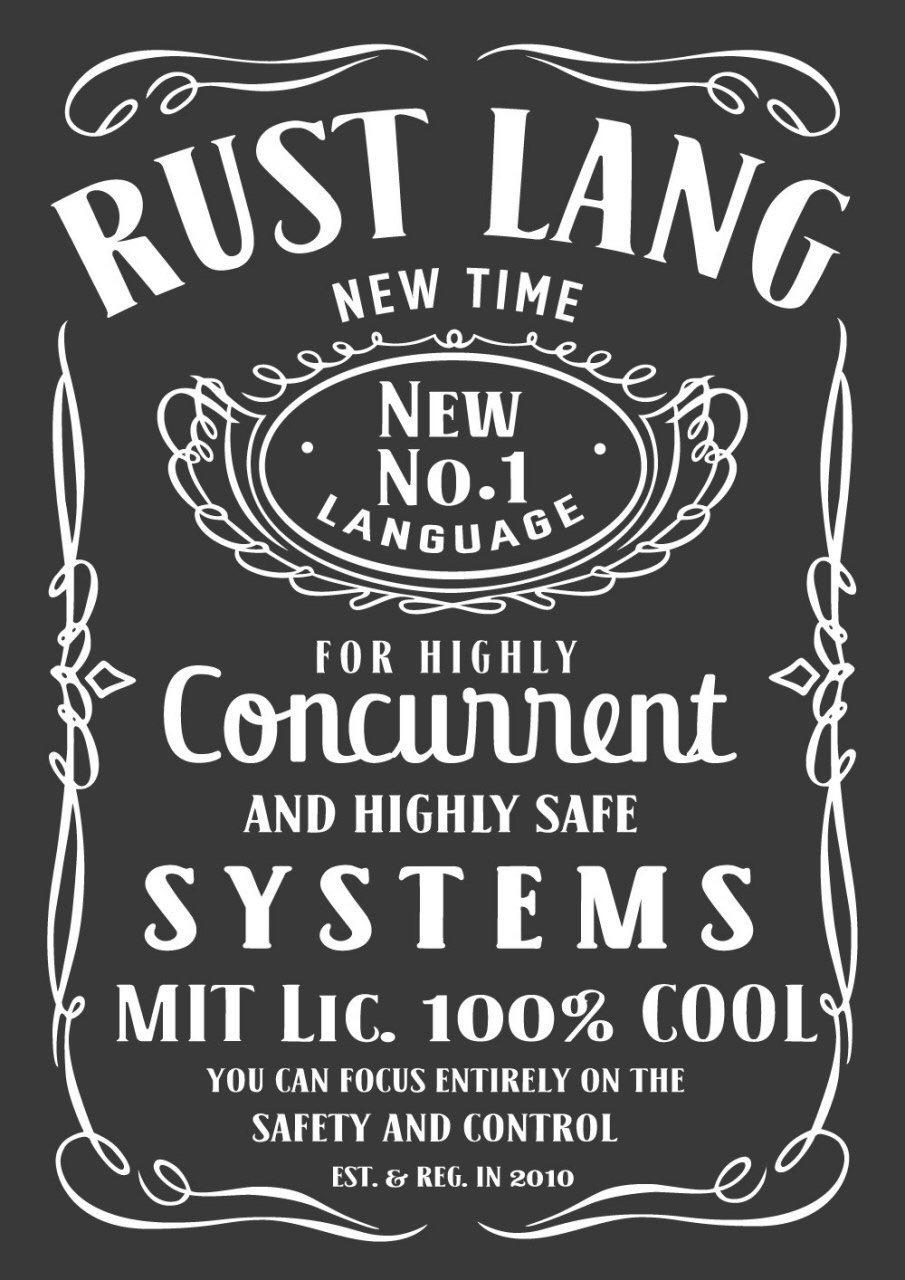
\includegraphics[height = 0.8\textheight]{rust_lang.jpg}
    \end{column}
    \begin{column}{0.6\textwidth}
      \begin{itemize}
      \item Performance
        \begin{itemize}
        \item Fast, memory-efficient
        \item No runtime or garbage collector
        \item Zero-cost abstractions
        \end{itemize}
      \item Reliability
        \begin{itemize}
        \item Rich type system
        \item Ownership model
        \end{itemize}
      \item Productivity
        \begin{itemize}
        \item Documentation
        \item Friendly compiler
        \item Top-notch tooling
        \end{itemize}
      \end{itemize}
    \end{column}
  \end{columns}

  \note{

    Какие характерные черты данного языка можно выделить?

    \begin{itemize}
    \item Быстрый за счёт \textbf{нулевой стоимости абстракций}, без GC, поэтому
      можно \textbf{встраивать в другие языки}, в \textbf{критические сервисы},
      запускать \textbf{на встраиваемых системах}.
    \item Богатая система типов и модель владения, отсюда --- \textbf{безопасная
        работа} с памятью и потоками, многие ошибки отлавливаются \textbf{во
        время компилирования}.
    \item Благодаря \textbf{дружелюбному сообществу} и \textbf{open-source
        разработке} у Rust много преимуществ.
    \end{itemize}

  }
\end{frame}
